\chapter{Theoretical and experimental basics}
\label{theory}

\section{The Standard Model of Particle Physics}

The Standard Model of Particle Physics summarizes the current knowledge of fundamental particles and their interactions. The model holds at scales of 1 fm and below. Gravity, being the fourth fundamental force is not included because it is negligible for most phenomena at this scale.

The current view is that all matter is made out of three kinds of elementary particles being leptons quarks and mediators.
There are six leptons falling into three families according to charge, electron number, muon number and tau number. 

Similiar to that there are six flavors of quarks separated by Strangeness (S), charm (C), Beauty (B), and truth (T). As well as the leptons the quarks fall into three generations.
For both kinds of particles the mass rises with the generations and every generation comes as a doublet. The first particle of each lepton doublet is not charged and referred to as a neutrino while the second particle has charge -1.
For each quark doublet there is an element with fractional charge $-\frac{1}{3}$ and an element with fractional charge $\frac{2}{3}$.
To every of these particles there is an anti particle with opposite charge.

The third kind of particle included in the standard model is the mediator. Mediators are gauge bosons whose exchange allows the particles to interact. There are four kinds of of elemtary interactions of which the strong electromagnetic and weak interaction are included in the model. The fourth interaction is the gravitational interaction.
The gauge particles for the strong interaction are the gluons carrying colour charge, the electromagnetic mediator is the photon ($\gamma$) and the weak mediators are the $W^{\pm}$ and $Z$ bosons.
Tables \ref{lepton properties}, \ref{quark properties} and \ref{mediator properties} summarize the particles and their important properties.
\newpage


\begin{table}[h]
\centering
\caption{Lepton properties}
\label{lepton properties}
\begin{tabular}{l|l|S|S|S|S|}
\cline{2-6}
                                   & symbol        & \text{Charge}  & \text{\ensuremath{L_e}} & \text{\ensuremath{L_{\mu}}} & \text{\ensuremath{L_{\tau}}} \\ \cline{2-6} 
\multirow{2}{*}{First generation\{}  & $e$             & -1       & 1    & 0          & 0           \\ \cline{2-6} 
                                   & $\nu_e$        & 0        & 1    & 0          & 0           \\ \cline{2-6} 
\multirow{2}{*}{Second generation\{} & $\mu$           & -1       & 0    & 1          & 0           \\ \cline{2-6} 
                                   & $\nu_{\mu}$  & 0        & 0    & 1          & 0           \\ \cline{2-6} 
\multirow{2}{*}{Third generation\{}  & $\tau$          & -1       & 0    & 0          & 1           \\ \cline{2-6} 
                                   & $\nu_{\tau}$ & 0        & 0    & 0          & 1           \\ \cline{2-6} 
\end{tabular}
\end{table}

\begin{table}[h]
\centering
\caption{Quark properties}
\label{quark properties}
\begin{tabular}{l|l|S|S|l|l|l|l|l|l|}
\cline{2-10}
                                      & Symbol & \text{Charge Q}      & \text{mass}       & D  & U & S  & C & B  & T \\ \cline{2-10} 
\multirow{2}{*}{First generation \{}  & $d$    &\text{\ensuremath{-\frac{1}{3}}} & \SI{4.8}{MeV}    & -1 & 0 & 0  & 0 & 0  & 0 \\ \cline{2-10} 
                                      & $u$    & \text{\ensuremath{\frac{2}{3}}}  & \SI{2.3}{MeV}   & 0  & 1 & 0  & 0 & 0  & 0 \\ \cline{2-10} 
\multirow{2}{*}{Second generation \{} & $s$    & \text{\ensuremath{-\frac{1}{3}}} & \SI{95}{MeV}    & 0  & 0 & -1 & 0 & 0  & 0 \\ \cline{2-10} 
                                      & $c$    & \text{\ensuremath{\frac{2}{3}}}  & \SI{1275}{MeV}   & 0  & 0 & 0  & 1 & 0  & 0 \\ \cline{2-10} 
\multirow{2}{*}{Third generation \{}  & $b$    & \text{\ensuremath{-\frac{1}{3}}} & \SI{4180}{MeV}   & 0  & 0 & 0  & 0 & -1 & 0 \\ \cline{2-10} 
                                      & $t$    & \text{\ensuremath{\frac{2}{3}}}  & \SI{173210}{MeV} & 0  & 0 & 0  & 0 & 0  & 1 \\ \cline{2-10} 
\end{tabular}
\end{table}

\begin{table}[h]
\centering
\caption{Mediator properties}
\label{mediator properties}
\begin{tabular}{|l|l|l|l|l|}
\hline
Interaction     & Theory & Mediator        & Charge          & Coupling  \\ \hline
Strong          & QCD    & gluons (8)      & colour          & 1         \\ \hline
Electromagnetic & QED    & photon $\gamma$ & electric charge & $10^{-1}$ \\ \hline
Weak            & GSW    & $W^{\pm}, Z$    & weak isospin    & $20^{-6}$ \\ \hline
\end{tabular}
\end{table}

Given this the standard model of particle physics has been a very successful model for a very long time and still holds for most cases.
Nevertheless the model has some commonly known weaknesses and does not claim to be complete. For example the gravitational force is not included and in the standard model neutrinos are massless.
The Higgs boson as the mediator of gravitation has been discovered at the LHC in 2012. 
For further information check \cite{griffith08}, \cite{thomson13} and \cite{brock11}.

Should there be an outline here ? 
\newpage





\section{The LHC and ATLAS}

The analysis for this thesis has been performed in the ATLAS collaboration. The ATLAS-Detector is one of the four big experiments at the LHC at Cern. Therefore this chapter gives a brief overview over the LHC and ATLAS focusing on the properties directly relevant for Particle Flow Analysis.

After a description of the ATLAS detector in general I will give a little bit more information about the detector components directly relevant for the explanation of particle flow being the tracking detector and the calorimeter. To make the advantages of particle flow understandable to the reader I will give a general description of these detectors and their properties irrespective of their detailed construction at ATLAS.

\subsection{The LHC}

The Large Hadron Collider ("LHC") is part of the facilities of the European Organization of Nuclear Research ("CERN") and was built to extend the frontiers of modern particle physics by delivering high luminosities and unprecedented high energies. The Collider is circular with a circumfence of \SI{26.659}{\km} and is located \SI{10}{\km} underground close to Geneva.\\
The LHC is designed to collide bunches of up to \num{d11} protons at a luminosity of \SI{d34}{\per\square\cm \per\s}. The beams are collided at four collision points being the four main experiments at the LHC. Tw of these are special-purpose detectors, namely LHCb and ALICE while the other two are general-purpose detectors.
The general-purpose experiments are CMS and ATLAS. The analysis in this thesis has been performed on ATLAS data.
Figure \ref{fig:LHC} shows the LHC, the four detectors and its general location.
\begin{figure}[h]
  \centering
  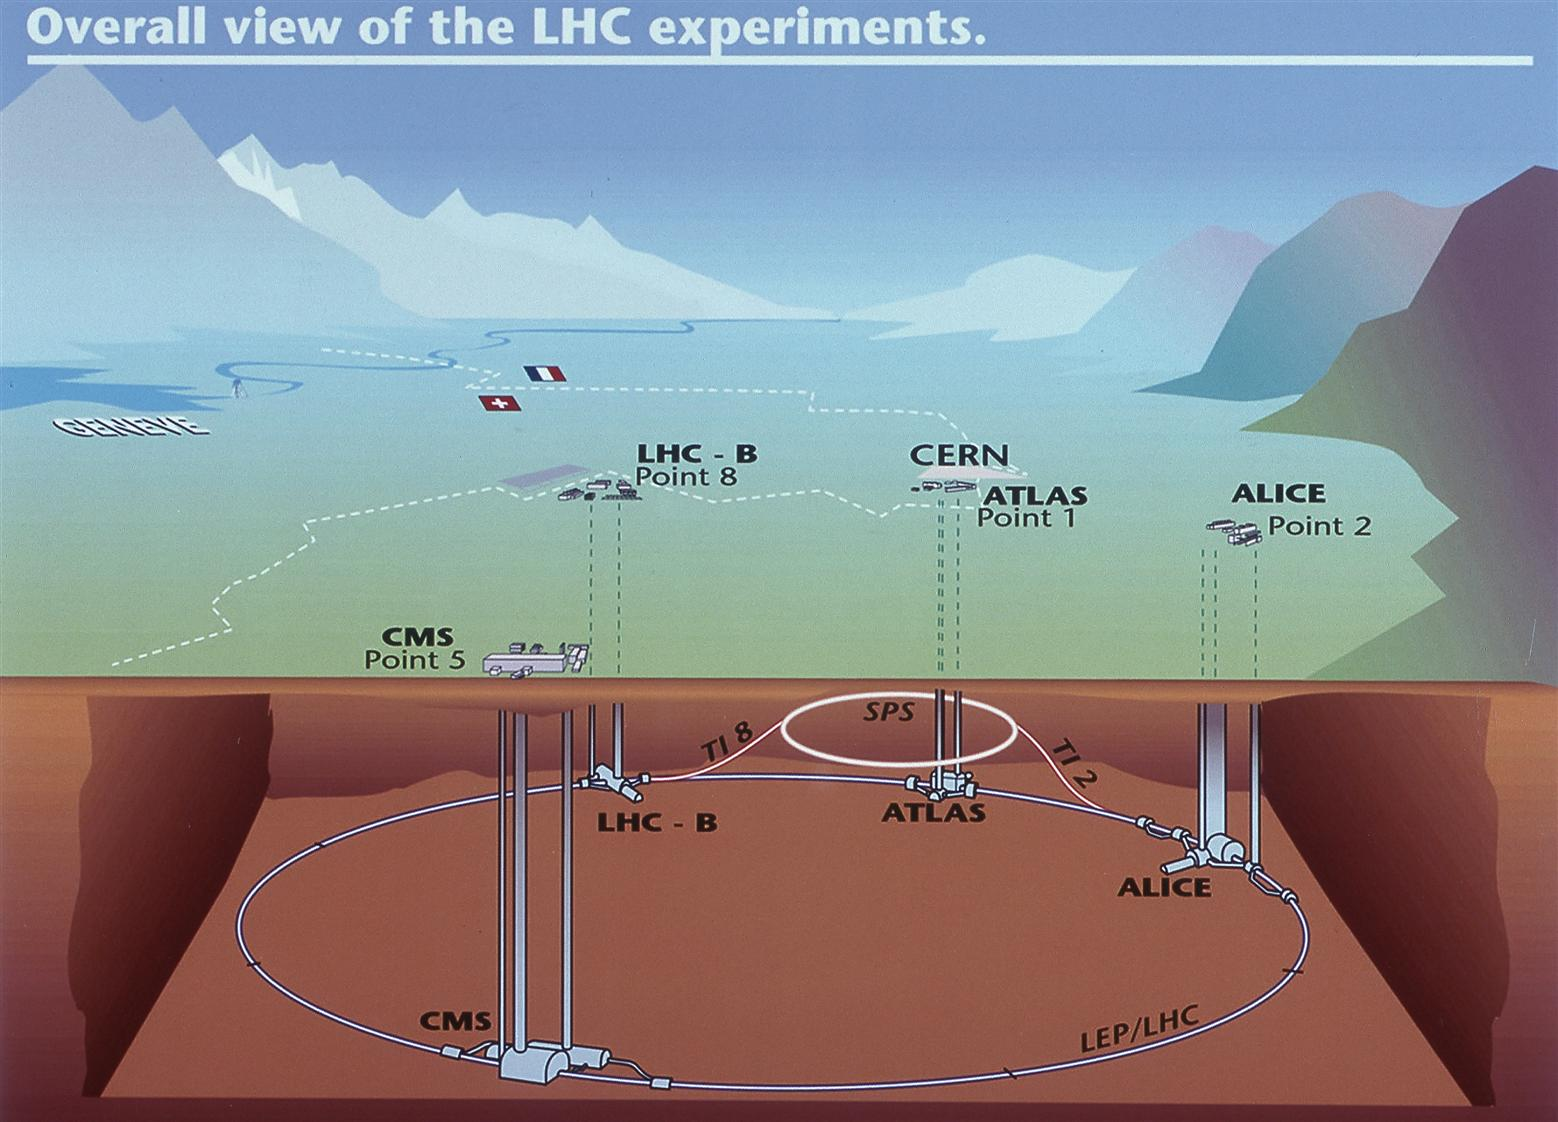
\includegraphics[width=\figwidth]{CERN_all-experiments}
  \caption[Sketch of the LHC ring, the position of the experiments and
  the surrounding countryside.]{Sketch of the LHC ring, the position
    of the experiments and the surrounding countryside. The four big
    LHC experiments are indicated. The location of the injection lines
    and the SPS are also shown. \cite{atlasfigures}}
  \label{fig:LHC}
\end{figure}


\subsection{The ATLAS Detector}

The ATLAS-Detector is built to take advantage of the high energy available at the LHC to observe highly massive particles that lower energy accelerators were not able to create and that way bring new physics theory beyond the standard model of particle physics.
It is designed to be able to observe a maximized number of final stages being a so called general purpose-detector. This means that the detector should be able to identify every kind of particle and still provide a accurate information about angle and momentum.
Figure \ref{fig:atlas} shows the outline of the ATLAS detector together with a rough scale in size. In the following explanations of the components from the inside to the outside are given.

\begin{figure}[h]
  \centering
  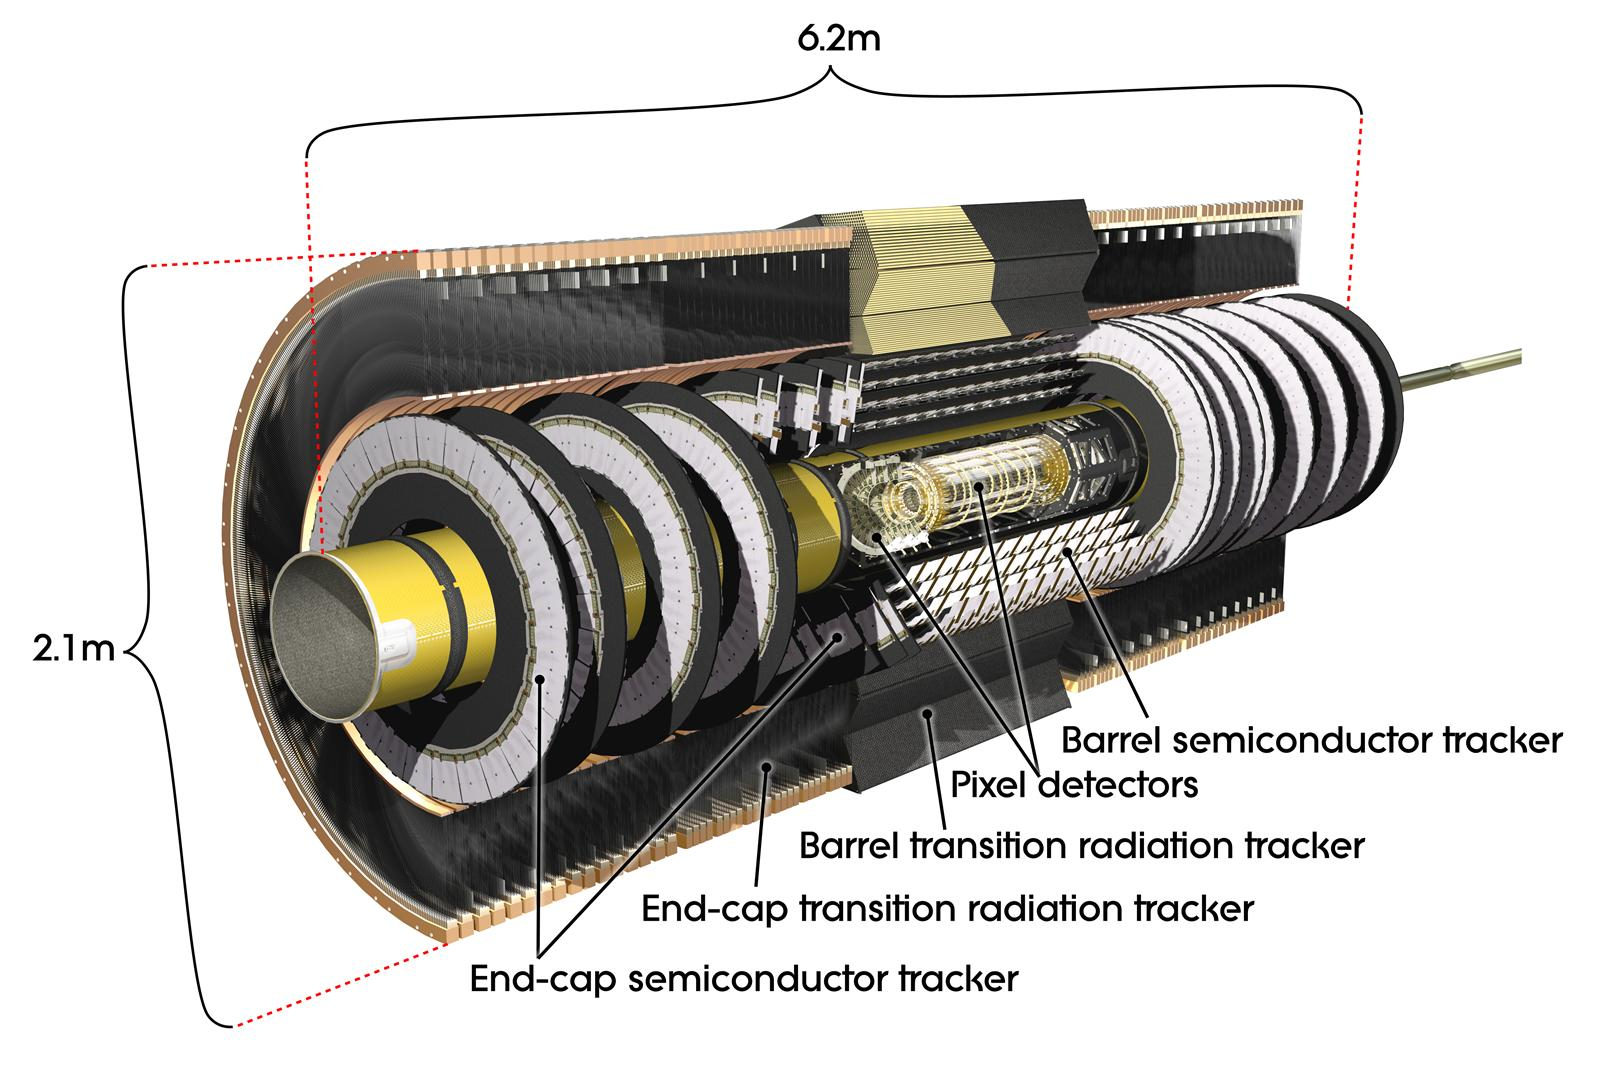
\includegraphics[width=\figwidth]{atlas-detector}
  \caption[Sketch of the ATLAS detector]{Sketch of the ATLAS detector \cite{atlasfigures}}
  \label{fig:atlas}
\end{figure}

Figure \ref{fig:atlas_sketch} shows the detector's components in a simplified way and allows to understand the order of the important detector parts in detail. The innermost part of the detector is a tracking detector in a field of a large solenoid coil to obtain charge and trajectory of charged particles.
The following two parts are the Electromagnetic and Hadronic Calorimeter which together build the Calorimeter part of the detector. One of them focuses on measuring the energy in electromagnetic showers while the other one is optimized for hadronic particle showers. The outermost part is a Muon spectrometer because most of the particles that cross the calorimeters undetected are muons.


\begin{figure}[h]
  \centering
  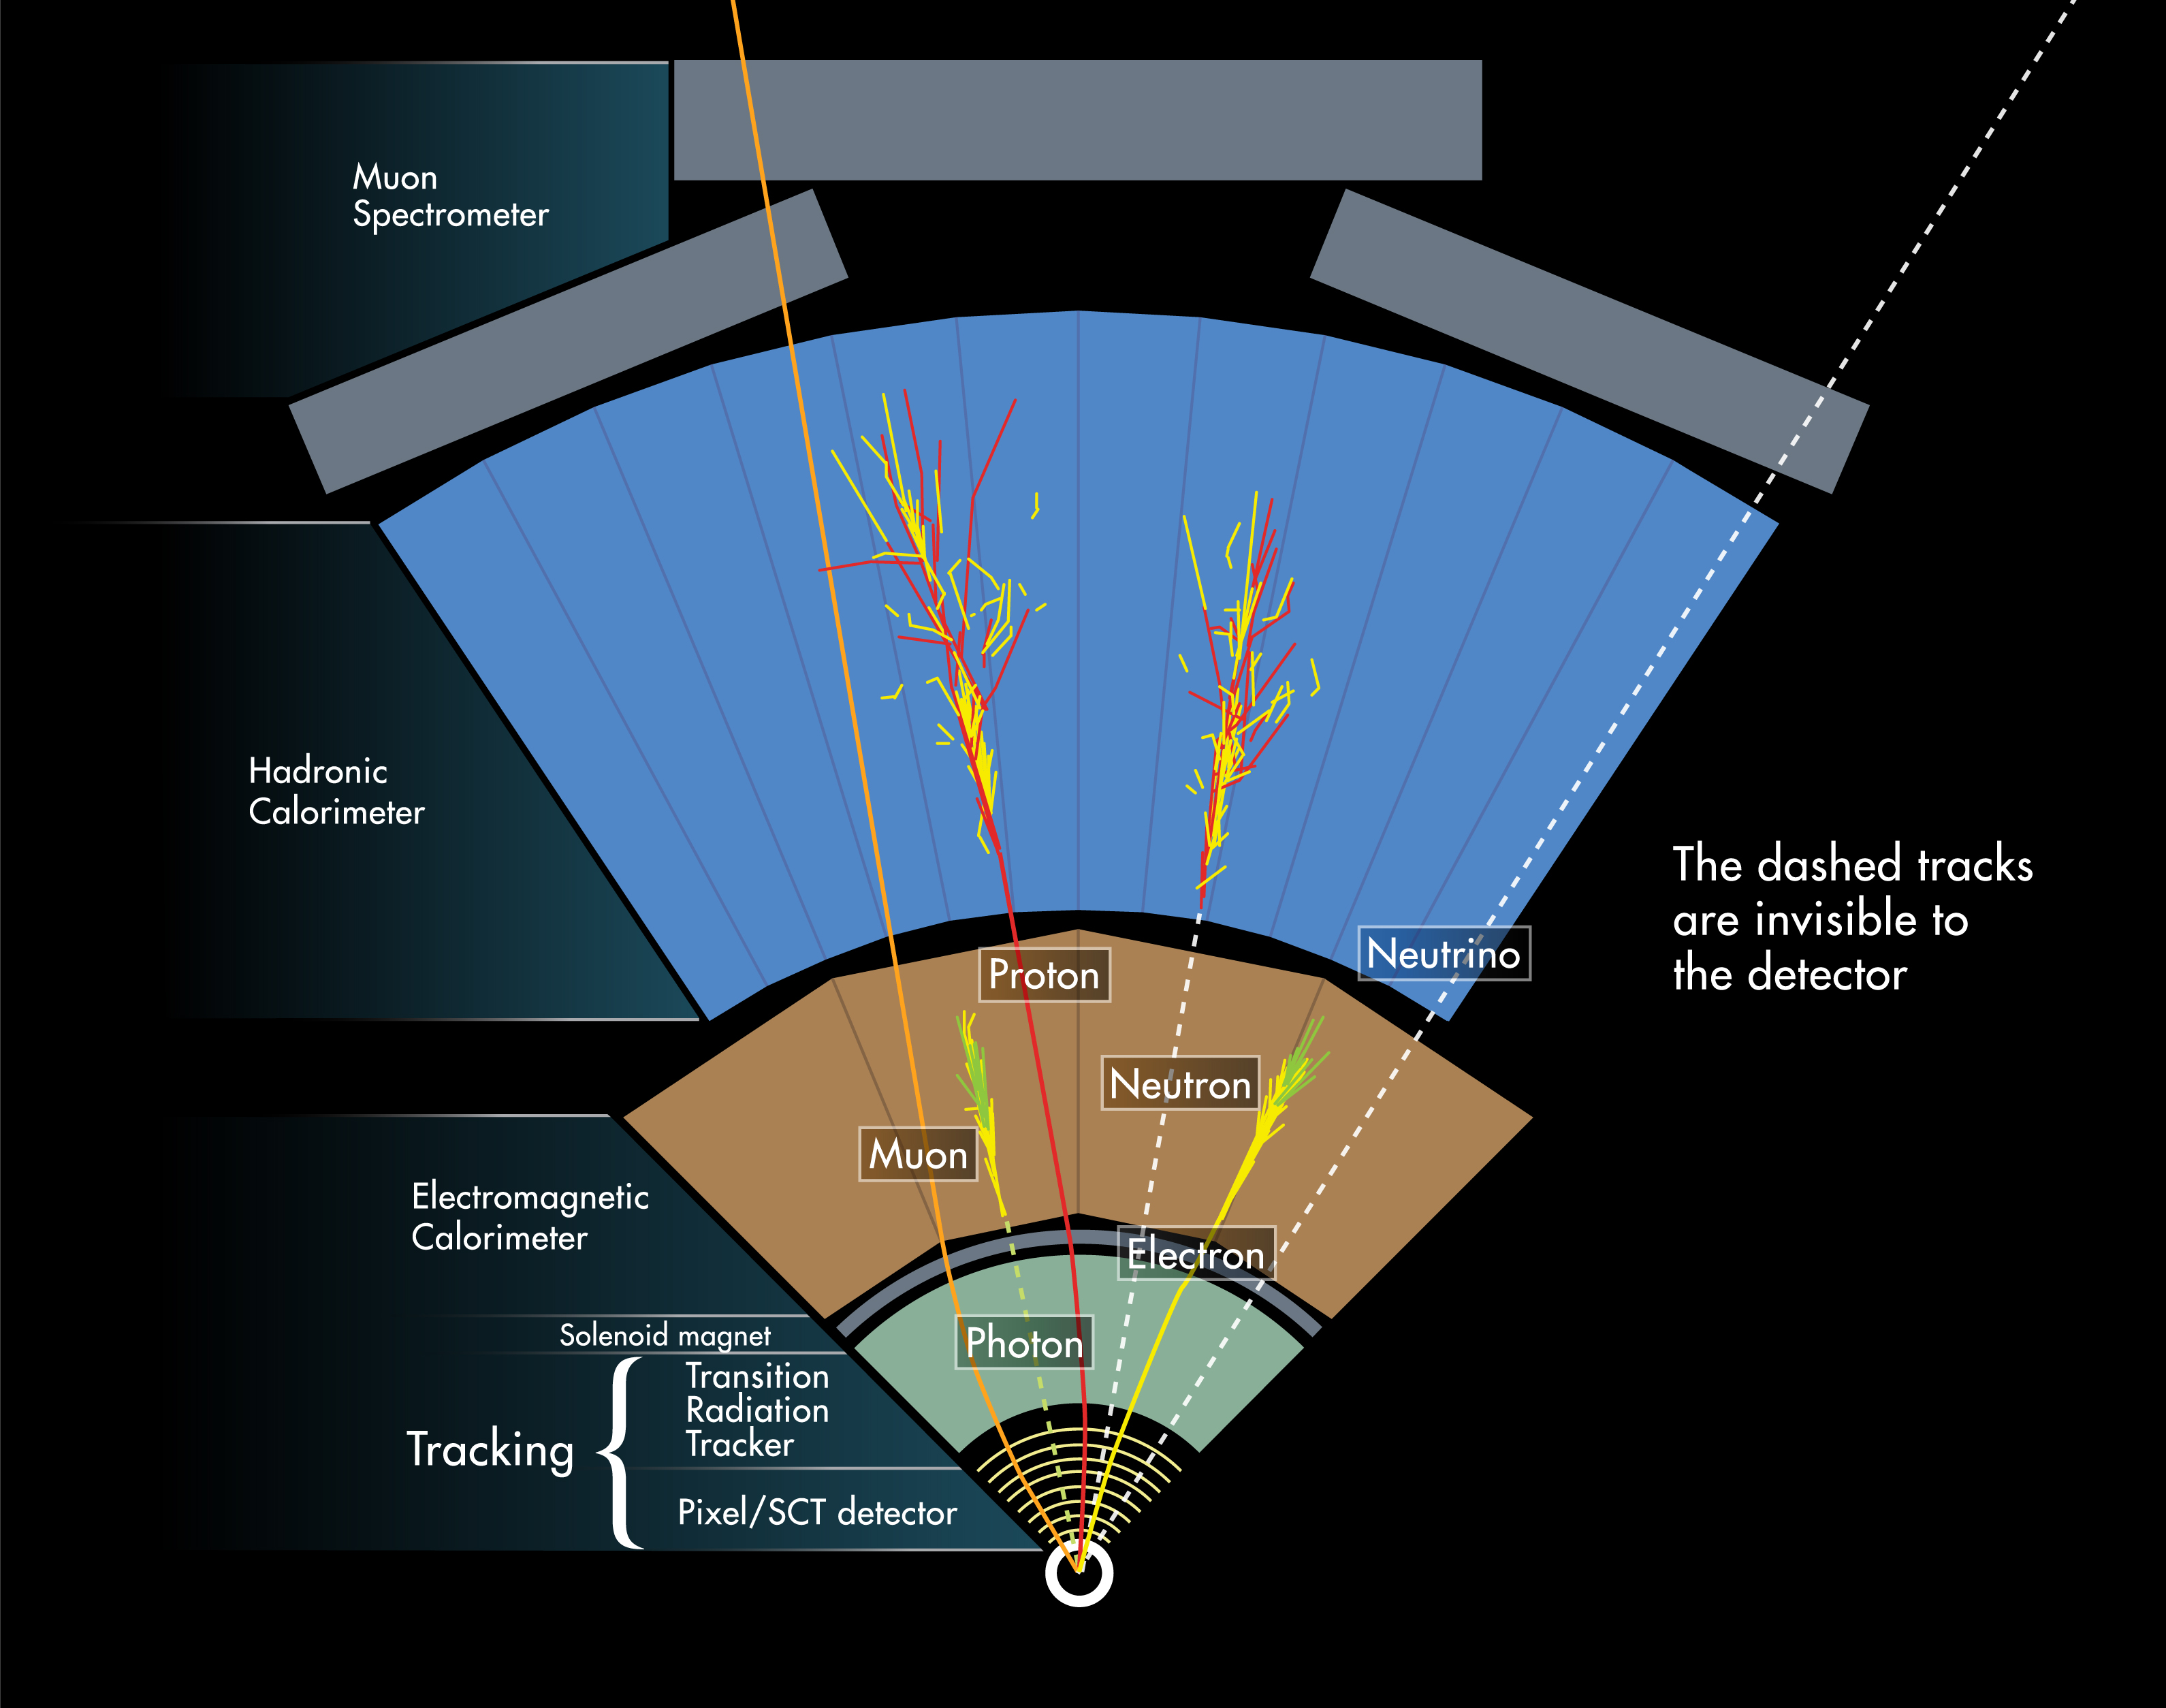
\includegraphics[width=\figwidth]{atlas-abstract}
  \caption[Sketch of the transversal section of the ATLAS detector]{Scheme of the ATLAS-detector \cite{atlasfigures}}
  \label{fig:atlas_sketch}
\end{figure}

\subsection{Tracking detectors}

The go to method to measure the momenta of charged particles is the usage of tracking detectors
These detectors are based on charged particles leaving a track of ionisations in any given medium and therefore by detecting this ionizations being able to reconstruct the particles trajectory.
There are two main categories for tracking detectors in use. The first one uses a large gaseous volume in a strong electric field and filled with a structure of wires. The electric field lets the liberating electrons drift towards the wires where they cause a detectable signal.

However the second kind of detectors is based on semiconductor technology and is used in most modern detectors like ATLAS. Therefore I will give this kind of tracking detectors a deeper discussion.
If a charged particle traverses a appropriately doped semiconductor wafer for example a doped silicon wafer it creates electron hole pairs along its trail. If an electric field is applied to the semiconductor material the holes will drift in the direction of the electric field and can then be collected by p-n junctions.

Usually a tracking detector is divided into semiconductor strips or pixel in a magnitude of $25 \mu m$. That way a signal at a certain junction can be used to reconstruct a trail and position. The common way to reconstruct a track is a set of cylindrical semiconductor wafers in a magnetic field. Each wafer signal gives a rough estimation of the particle's location at the time and the curve given by the sum of signals allows to calculate charge and momentum.

\begin{equation}
p \cdot cos \lambda = 0.3 BR
\end{equation}

%I need graphics here for sure

\subsubsection{Inner Detector}

The Tracking detectors of the ATLAS detector are called the Inner Detector. It consists of three sub-components being the Pixel detector (Pixel), the Semi-Conductor Tracker (SCT) and a Transition Radiation Tracker (TRT). Each one of this sub-detectors is divided in a barrel part and two end-caps. The Inner detector covers a region of $|\eta| < 2.5$ which also limits the region in which particle flow can be used.

\subsubsection{Muon spectrometer}

The outermost part of the detector are the Muon tracking chambers or the so calles muon spectrometer. The task of the spectrometer is to detect charged particles transversing the calorimeter undetected and to both trigger on them and to measure their energy. Due to these two functions the spectromeer is divided into two parts each dedicated to one of the tasks. The first part is the trigger chamber covering a range of $|\eta|<2.4$ and with a range of $|\eta|<2.7$ comes the high-precision chamber as the second part. The main detectors support feet cause a further gap at about $\phi = \ang{300}$ and $\phi = \ang{270}$. 

The hih-precision detector uses Monitored Drift Tubes (MDTs) while the trigger chamber uses Resistive-Plate Chambers (RPCs). The momentum calculation then is performed by the field of the torroid magnet.

%get more from Jan thesis


\subsection{Calorimeter}

In particle physics a calorimeter is a device to measure first and foremost the total energy of a particle. Most of the time also some positional information is taken.
The idea is that most particles loose all their momentum crossing the calorimeter-structure. Measuring the energy deposited this way gives a measurement for the particle's energy.
Usually a particle deposits its energy by initiating a particle shower. the shower's energy is then collected and measured.
Calorimeters are distinguished by the main interaction of the particles one wants to detect. 
\subsubsection{Electromgnetic Calorimeter}

Electromagnetic calorimeters are designed to detect charged particles and measure their total energy. Usually these particles are electrons and photons. There are various methods to construct these detectors. An example would be the usage of inorganic scintillators. These scintillators should be optically transparent and have a short radiation length to contain the shower in a compact region. The detection then can follow by photon detectors which measure the radiation light being proportional to the detected particle's energy. The energy resolution of these detectors is typically in the range

\begin{equation}
\frac{\sigma_E}{E} \sim \frac{3 \% - 10 \%}{\sqrt{E/GeV}}.
\end{equation}

The electromagnetic calorimeter at ATLAS is a high-resolution and high-granularity liquid-argon sampling calorimeter. Leas is used as absorber material. The calorimeter consists of two half-barrels which are only divided by a small gap at the interaction point. The endcaps at each side are segmented into two coaxial wheels to cover different polar angles.

\subsubsection{Hadronic calorimeters}

Hadronic calorimeters are used to obtain the energies of hadronic particle showers.
Due to the relatively large distance between interactions these calorimeters occupy a significantly large space in the detector.

A common technique to construct these calorimeters is a sandwich like structure of alternating layers of high density absorber material and active material. 
The absorbers are used to develop the particle showers which then hit the active material and deposit the energy there. That way hadronic calorimeters reach a resolution of about

\begin{equation}
\frac{\sigma_E}{E} \gtrsim \frac{50 \%}{\sqrt{E/GeV}}.
\end{equation}


For more information see the ATLAS design report \cite{atlastdr}

